\section{文献小结}

\subsection{研究内容分类}
\begin{frame}{研究内容分类}
    按研究方法分类:
    \begin{itemize}
        \item 传统超分方法研究
        \item 深度学习超分方法研究
    \end{itemize}
    \vspace{1cm}
    按有无具体应用分类:
    \begin{itemize}
        \item 纯方法研究
        \item 具体应用相关
    \end{itemize}
\end{frame}

\begin{frame}{传统超分方法研究}
    ~\cite{guoxx}, ~\cite{zhaoxd}, ~\cite{liaoxx}, ~\cite{xuy}和~\cite{liz}等文献
    
    其论文内容包括如下: 
    \begin{itemize}
        \item 图像处理方法研究, 如匹配, 角点检测等 
        \item 针对传统超分算法的改进
        \item 针对序列图像超分算法的改进
    \end{itemize}

    以~\cite{zhaoxd}为例, 其论文内容为:
    \begin{itemize}
        \item 多幅图像配准算法及其并行化设计方法
        \item 结合非线性各向异性张量扩散和改进梯度矢量流连续性约束的双正则项多帧超分算法
        \item 改进初始聚类中心的K-PCA自适应字典学习算法的单帧超分算法
        \item 基于偏微分方程统一框架的单帧超分算法
    \end{itemize}
\end{frame}

\begin{frame}{基于深度学习的超分方法研究}
    ~\cite{wangyf}, ~\cite{zhengk}和~\cite{fengxb}等文献

    其论文内容包括如下:
    \begin{itemize}
        \item 针对某一问题, 更改网络结构或损失函数
        \item 针对某一种网络, 更改网络结构或损失函数
        \item 改变训练方式降低对数据集要求
    \end{itemize}

    以~\cite{fengxb}为例, 其论文内容:
    \begin{itemize}
        \item 基于卷积网络改进的超分方法
        \item 基于GAN改进的超分方法
        \item 无监督的超分方法
    \end{itemize}    
\end{frame}

\subsection{具体研究内容}

\begin{frame}{纯方法研究}
    多个研究内容并无核心突出某一问题

    单对方法进行改进
    \begin{itemize}
        \item ~\cite{guoxx}
        \item ~\cite{zhaoxd}
        \item ~\cite{liz}
    \end{itemize}

    以~\cite{fengxb}为例, 其论文内容:
    \begin{itemize}
        \item 基于卷积网络改进的超分方法
        \item 基于GAN改进的超分方法
        \item 无监督的超分方法
    \end{itemize}    

\end{frame}

\begin{frame}{针对某一问题}

    从论文结构中能明显看到研究内容围绕一个核心点展开
    \begin{itemize}
        \item ~\cite{zhengk} 将研究内容聚焦在高光谱影像与分类
        \item ~\cite{huxc} 将研究内容集中在自适应分辨率
    \end{itemize}
    以~\cite{zhengk}为例:
    
    其论文研究内容:
    \begin{itemize}
        \item 基于卷积网络单张高光谱超分方法研究
        \item 基于深度学习高光谱和多光谱非监督超分方法
        \item 多尺度空谱特征的高光谱影像分类研究
        \item 超分后高光谱分类研究
    \end{itemize}
\end{frame}



% \begin{frame}{可用哨兵数据空间位置}
%     \small
%     考虑到六幅影像的范围有重叠, 只用其中一组即可
%     \begin{figure}
%         \centering
%         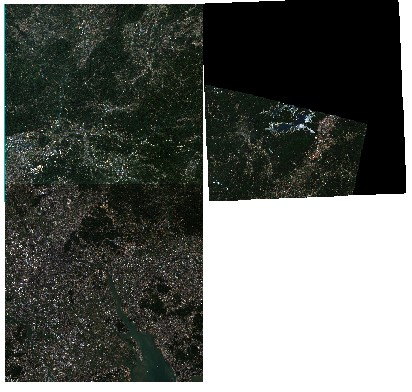
\includegraphics[width=6cm]{pic/pic0115.jpg}
%         \caption{哨兵可用重叠}
%         \label{fig:0109}
%     \end{figure}
% \end{frame}

% \begin{frame}{数据查询}
%     \begin{columns}
%         \column{0.3\textwidth}
%         \begin{itemize}
%             \item \small{对广东区域进行影像检索}
%         \end{itemize}

%         \column{0.7\textwidth}
%         \begin{figure}
%             \centering
%             % Requires \usepackage{graphicx}
%             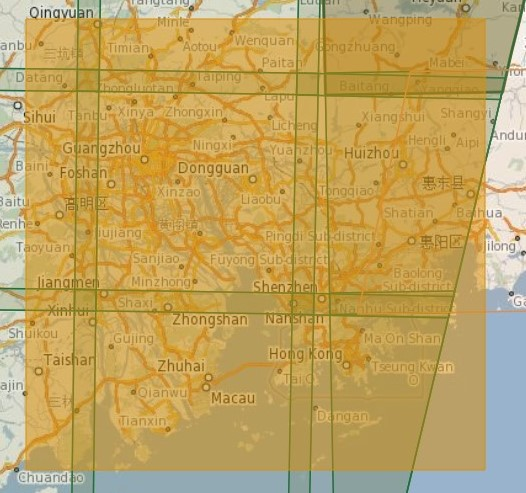
\includegraphics[width=5cm]{pic/pic0101.jpg}
%             \caption{影像查询地区}
%             \label{fig:0101}
%         \end{figure}
%     \end{columns}
% \end{frame}